% !TEX encoding = UTF-8 Unicode
%% bare_conf_compsoc.tex
%% V1.4b
%% 2015/08/26
%% by Michael Shell
%% See:
%% http://www.michaelshell.org/
%% for current contact information.
%%
%% This is a skeleton file demonstrating the use of IEEEtran.cls
%% (requires IEEEtran.cls version 1.8b or later) with an IEEE Computer
%% Society conference paper.
%%
%% Support sites:
%% http://www.michaelshell.org/tex/ieeetran/
%% http://www.ctan.org/pkg/ieeetran
%% and
%% http://www.ieee.org/

%%*************************************************************************
%% Legal Notice:
%% This code is offered as-is without any warranty either expressed or
%% implied; without even the implied warranty of MERCHANTABILITY or
%% FITNESS FOR A PARTICULAR PURPOSE! 
%% User assumes all risk.
%% In no event shall the IEEE or any contributor to this code be liable for
%% any damages or losses, including, but not limited to, incidental,
%% consequential, or any other damages, resulting from the use or misuse
%% of any information contained here.
%%
%% All comments are the opinions of their respective authors and are not
%% necessarily endorsed by the IEEE.
%%
%% This work is distributed under the LaTeX Project Public License (LPPL)
%% ( http://www.latex-project.org/ ) version 1.3, and may be freely used,t
%% distributed and modified. A copy of the LPPL, version 1.3, is included
%% in the base LaTeX documentation of all distributions of LaTeX released
%% 2003/12/01 or later.
%% Retain all contribution notices and credits.
%% ** Modified files should be clearly indicated as such, including  **
%% ** renaming them and changing author support contact information. **
%%*************************************************************************


% *** Authors should verify (and, if needed, correct) their LaTeX system  ***
% *** with the testflow diagnostic prior to trusting their LaTeX platform ***
% *** with production work. The IEEE's font choices and paper sizes can   ***
% *** trigger bugs that do not appear when using other class files.       ***                          ***
% The testflow support page is at:
% http://www.michaelshell.org/tex/testflow/



\documentclass[conference,compsoc]{IEEEtran}
% Some/most Computer Society conferences require the compsoc mode option,
% but others may want the standard conference format.
%
% If IEEEtran.cls has not been installed into the LaTeX system files,
% manually specify the path to it like:
% \documentclass[conference,compsoc]{../sty/IEEEtran}





% Some very useful LaTeX packages include:
% (uncomment the ones you want to load)


% *** MISC UTILITY PACKAGES ***
%
%\usepackage{ifpdf}
% Heiko Oberdiek's ifpdf.sty is very useful if you need conditional
% compilation based on whether the output is pdf or dvi.
% usage:
% \ifpdf
%   % pdf code
% \else
%   % dvi code
% \fi
% The latest version of ifpdf.sty can be obtained from:
% http://www.ctan.org/pkg/ifpdf
% Also, note that IEEEtran.cls V1.7 and later provides a builtin
% \ifCLASSINFOpdf conditional that works the same way.
% When switching from latex to pdflatex and vice-versa, the compiler may
% have to be run twice to clear warning/error messages.


\usepackage[utf8]{inputenc}
\usepackage[portuguese]{babel}

\usepackage{url}
\usepackage{hyperref} 
\usepackage{graphicx}
\usepackage{fancyref}
\usepackage{amsmath}
\usepackage{float}
\usepackage{fancyhdr}
\pagestyle{fancy}

\usepackage{listings,mdframed}


\lstset{
	language=c,
	keywordstyle=\bfseries\ttfamily\color[rgb]{0,0,1},
	identifierstyle=\ttfamily,
	commentstyle=\color[rgb]{0.133,0.545,0.133},
	stringstyle=\ttfamily\color[rgb]{0.627,0.126,0.941},
	showstringspaces=false,
	basicstyle=\tiny,
numberstyle=\tiny,
numbers=right,
	stepnumber=1,
	numbersep=10pt,
	tabsize=1,
	breaklines=true,
	prebreak = \raisebox{0ex}[0ex][0ex]{\ensuremath{\hookleftarrow}},
	breakatwhitespace=false,
	aboveskip={1.5\baselineskip},
  columns=fixed,
  upquote=true,
  extendedchars=true,
 frame=single,
 inputencoding=utf8,
    literate={á}{{\'a}}1 {ã}{{\~a}}1 {â}{{\~a}}1 {é}{{\'e}}1 {ê}{{\'e}}1 {ç}{{\'c}}1 {ú}{{\'u}}1 {ó}{{\'o}}1 {í}{{\'i}}1,
 %backgroundcolor=\color{lbcolor},
}

% *** CITATION PACKAGES ***
%
\ifCLASSOPTIONcompsoc
  % IEEE Computer Society needs nocompress option
  % requires cite.sty v4.0 or later (November 2003)
  \usepackage[nocompress]{cite}
\else
  % normal IEEE
  \usepackage{cite}
\fi
% cite.sty was written by Donald Arseneau
% V1.6 and later of IEEEtran pre-defines the format of the cite.sty package
% \cite{} output to follow that of the IEEE. Loading the cite package will
% result in citation numbers being automatically sorted and properly
% "compressed/ranged". e.g., [1], [9], [2], [7], [5], [6] without using
% cite.sty will become [1], [2], [5]--[7], [9] using cite.sty. cite.sty's
% \cite will automatically add leading space, if needed. Use cite.sty's
% noadjust option (cite.sty V3.8 and later) if you want to turn this off
% such as if a citation ever needs to be enclosed in parenthesis.
% cite.sty is already installed on most LaTeX systems. Be sure and use
% version 5.0 (2009-03-20) and later if using hyperref.sty.
% The latest version can be obtained at:
% http://www.ctan.org/pkg/cite
% The documentation is contained in the cite.sty file itself.
%
% Note that some packages require special options to format as the Computer
% Society requires. In particular, Computer Society  papers do not use
% compressed citation ranges as is done in typical IEEE papers
% (e.g., [1]-[4]). Instead, they list every citation separately in order
% (e.g., [1], [2], [3], [4]). To get the latter we need to load the cite
% package with the nocompress option which is supported by cite.sty v4.0
% and later.





% *** GRAPHICS RELATED PACKAGES ***
%
\ifCLASSINFOpdf
  % \usepackage[pdftex]{graphicx}
  % declare the path(s) where your graphic files are
  % \graphicspath{{../pdf/}{../jpeg/}}
  % and their extensions so you won't have to specify these with
  % every instance of \includegraphics
  % \DeclareGraphicsExtensions{.pdf,.jpeg,.png}
\else
  % or other class option (dvipsone, dvipdf, if not using dvips). graphicx
  % will default to the driver specified in the system graphics.cfg if no
  % driver is specified.
  % \usepackage[dvips]{graphicx}
  % declare the path(s) where your graphic files are
  % \graphicspath{{../eps/}}
  % and their extensions so you won't have to specify these with
  % every instance of \includegraphics
  % \DeclareGraphicsExtensions{.eps}
\fi
% graphicx was written by David Carlisle and Sebastian Rahtz. It is
% required if you want graphics, photos, etc. graphicx.sty is already
% installed on most LaTeX systems. The latest version and documentation
% can be obtained at: 
% http://www.ctan.org/pkg/graphicx
% Another good source of documentation is "Using Imported Graphics in
% LaTeX2e" by Keith Reckdahl which can be found at:
% http://www.ctan.org/pkg/epslatex
%
% latex, and pdflatex in dvi mode, support graphics in encapsulated
% postscript (.eps) format. pdflatex in pdf mode supports graphics
% in .pdf, .jpeg, .png and .mps (metapost) formats. Users should ensure
% that all non-photo figures use a vector format (.eps, .pdf, .mps) and
% not a bitmapped formats (.jpeg, .png). The IEEE frowns on bitmapped formats
% which can result in "jaggedy"/blurry rendering of lines and letters as
% well as large increases in file sizes.
%
% You can find documentation about the pdfTeX application at:
% http://www.tug.org/applications/pdftex





% *** MATH PACKAGES ***
%
%\usepackage{amsmath}
% A popular package from the American Mathematical Society that provides
% many useful and powerful commands for dealing with mathematics.
%
% Note that the amsmath package sets \interdisplaylinepenalty to 10000
% thus preventing page breaks from occurring within multiline equations. Use:
%\interdisplaylinepenalty=2500
% after loading amsmath to restore such page breaks as IEEEtran.cls normally
% does. amsmath.sty is already installed on most LaTeX systems. The latest
% version and documentation can be obtained at:
% http://www.ctan.org/pkg/amsmath





% *** SPECIALIZED LIST PACKAGES ***
%
%\usepackage{algorithmic}
% algorithmic.sty was written by Peter Williams and Rogerio Brito.
% This package provides an algorithmic environment fo describing algorithms.
% You can use the algorithmic environment in-text or within a figure
% environment to provide for a floating algorithm. Do NOT use the algorithm
% floating environment provided by algorithm.sty (by the same authors) or
% algorithm2e.sty (by Christophe Fiorio) as the IEEE does not use dedicated
% algorithm float types and packages that provide these will not provide
% correct IEEE style captions. The latest version and documentation of
% algorithmic.sty can be obtained at:
% http://www.ctan.org/pkg/algorithms
% Also of interest may be the (relatively newer and more customizable)
% algorithmicx.sty package by Szasz Janos:
% http://www.ctan.org/pkg/algorithmicx




% *** ALIGNMENT PACKAGES ***
%
%\usepackage{array}
% Frank Mittelbach's and David Carlisle's array.sty patches and improves
% the standard LaTeX2e array and tabular environments to provide better
% appearance and additional user controls. As the default LaTeX2e table
% generation code is lacking to the point of almost being broken with
% respect to the quality of the end results, all users are strongly
% advised to use an enhanced (at the very least that provided by array.sty)
% set of table tools. array.sty is already installed on most systems. The
% latest version and documentation can be obtained at:
% http://www.ctan.org/pkg/array


% IEEEtran contains the IEEEeqnarray family of commands that can be used to
% generate multiline equations as well as matrices, tables, etc., of high
% quality.




% *** SUBFIGURE PACKAGES ***
%\ifCLASSOPTIONcompsoc
%  \usepackage[caption=false,font=footnotesize,labelfont=sf,textfont=sf]{subfig}
%\else
%  \usepackage[caption=false,font=footnotesize]{subfig}
%\fi
% subfig.sty, written by Steven Douglas Cochran, is the modern replacement
% for subfigure.sty, the latter of which is no longer maintained and is
% incompatible with some LaTeX packages including fixltx2e. However,
% subfig.sty requires and automatically loads Axel Sommerfeldt's caption.sty
% which will override IEEEtran.cls' handling of captions and this will result
% in non-IEEE style figure/table captions. To prevent this problem, be sure
% and invoke subfig.sty's "caption=false" package option (available since
% subfig.sty version 1.3, 2005/06/28) as this is will preserve IEEEtran.cls
% handling of captions.
% Note that the Computer Society format requires a sans serif font rather
% than the serif font used in traditional IEEE formatting and thus the need
% to invoke different subfig.sty package options depending on whether
% compsoc mode has been enabled.
%
% The latest version and documentation of subfig.sty can be obtained at:
% http://www.ctan.org/pkg/subfig




% *** FLOAT PACKAGES ***
%
%\usepackage{fixltx2e}
% fixltx2e, the successor to the earlier fix2col.sty, was written by
% Frank Mittelbach and David Carlisle. This package corrects a few problems
% in the LaTeX2e kernel, the most notable of which is that in current
% LaTeX2e releases, the ordering of single and double column floats is not
% guaranteed to be preserved. Thus, an unpatched LaTeX2e can allow a
% single column figure to be placed prior to an earlier double column
% figure.
% Be aware that LaTeX2e kernels dated 2015 and later have fixltx2e.sty's
% corrections already built into the system in which case a warning will
% be issued if an attempt is made to load fixltx2e.sty as it is no longer
% needed.
% The latest version and documentation can be found at:
% http://www.ctan.org/pkg/fixltx2e


%\usepackage{stfloats}
% stfloats.sty was written by Sigitas Tolusis. This package gives LaTeX2e
% the ability to do double column floats at the bottom of the page as well
% as the top. (e.g., "\begin{figure*}[!b]" is not normally possible in
% LaTeX2e). It also provides a command:
%\fnbelowfloat
% to enable the placement of footnotes below bottom floats (the standard
% LaTeX2e kernel puts them above bottom floats). This is an invasive package
% which rewrites many portions of the LaTeX2e float routines. It may not work
% with other packages that modify the LaTeX2e float routines. The latest
% version and documentation can be obtained at:
% http://www.ctan.org/pkg/stfloats
% Do not use the stfloats baselinefloat ability as the IEEE does not allow
% \baselineskip to stretch. Authors submitting work to the IEEE should note
% that the IEEE rarely uses double column equations and that authors should try
% to avoid such use. Do not be tempted to use the cuted.sty or midfloat.sty
% packages (also by Sigitas Tolusis) as the IEEE does not format its papers in
% such ways.
% Do not attempt to use stfloats with fixltx2e as they are incompatible.
% Instead, use Morten Hogholm'a dblfloatfix which combines the features
% of both fixltx2e and stfloats:
%
% \usepackage{dblfloatfix}
% The latest version can be found at:
% http://www.ctan.org/pkg/dblfloatfix




% *** PDF, URL AND HYPERLINK PACKAGES ***
%
%\usepackage{url}
% url.sty was written by Donald Arseneau. It provides better support for
% handling and breaking URLs. url.sty is already installed on most LaTeX
% systems. The latest version and documentation can be obtained at:
% http://www.ctan.org/pkg/url
% Basically, \url{my_url_here}.




% *** Do not adjust lengths that control margins, column widths, etc. ***
% *** Do not use packages that alter fonts (such as pslatex).         ***
% There should be no need to do such things with IEEEtran.cls V1.6 and later.
% (Unless specifically asked to do so by the journal or conference you plan
% to submit to, of course. )


% correct bad hyphenation here
\hyphenation{op-tical net-works semi-conduc-tor}


\begin{document}
%
% paper title
% Titles are generally capitalized except for words such as a, an, and, as,
% at, but, by, for, in, nor, of, on, or, the, to and up, which are usually
% not capitalized unless they are the first or last word of the title.
% Linebreaks \\ can be used within to get better formatting as desired.
% Do not put math or special symbols in the title.
\title{Exercícios sobre a Ferramenta Dtrace}


% author names and affiliations
% use a multiple column layout for up to three different
% affiliations
\author{\IEEEauthorblockN{Sérgio Caldas}
\IEEEauthorblockA{Universidade do Minho\\Escola de Engenharia\\Departamento de Informática\\
Email: a57779@alunos.uminho.pt}}

% conference papers do not typically use \thanks and this command
% is locked out in conference mode. If really needed, such as for
% the acknowledgment of grants, issue a \IEEEoverridecommandlockouts
% after \documentclass

% for over three affiliations, or if they all won't fit within the width
% of the page (and note that there is less available width in this regard for
% compsoc conferences compared to traditional conferences), use this
% alternative format:
% 
%\author{\IEEEauthorblockN{Michael Shell\IEEEauthorrefmark{1},
%Homer Simpson\IEEEauthorrefmark{2},
%James Kirk\IEEEauthorrefmark{3}, 
%Montgomery Scott\IEEEauthorrefmark{3} and
%Eldon Tyrell\IEEEauthorrefmark{4}}
%\IEEEauthorblockA{\IEEEauthorrefmark{1}School of Electrical and Computer Engineering\\
%Georgia Institute of Technology,
%Atlanta, Georgia 30332--0250\\ Email: see http://www.michaelshell.org/contact.html}
%\IEEEauthorblockA{\IEEEauthorrefmark{2}Twentieth Century Fox, Springfield, USA\\
%Email: homer@thesimpsons.com}
%\IEEEauthorblockA{\IEEEauthorrefmark{3}Starfleet Academy, San Francisco, California 96678-2391\\
%Telephone: (800) 555--1212, Fax: (888) 555--1212}
%\IEEEauthorblockA{\IEEEauthorrefmark{4}Tyrell Inc., 123 Replicant Street, Los Angeles, California 90210--4321}}




% use for special paper notices
%\IEEEspecialpapernotice{(Invited Paper)}




% make the title area
\maketitle
\tableofcontents
\vspace{0.5cm}
% As a general rule, do not put math, special symbols or citations
% in the abstract
\begin{abstract}
Este relatório, exprime os resultados obtidos na resolução de exercícios sobre \textit{Dtrace}, no âmbito da disciplina de Engenharia de Sistemas de Comuptação (ESC), inserida no perfil de Computação Paralela e Distribuída (CPD) do curso de Engenharia Informática. O objetivo deste trabalho é praticar o uso do \textit{Dtrace}, numa máquina \textit{Soláris 11}, para isso foram propostos dois exercícios, sendo que os seus resultados são apresentados ao longo deste relatório. 
\end{abstract}

% no keywords




% For peer review papers, you can put extra information on the cover
% page as needed:
% \ifCLASSOPTIONpeerreview
% \begin{center} \bfseries EDICS Category: 3-BBND \end{center}
% \fi
%
% For peerreview papers, this IEEEtran command inserts a page break and
% creates the second title. It will be ignored for other modes.
\IEEEpeerreviewmaketitle



\section{Introdução}
Como foi dito anteriormente, foram propostos dois exercícios para a praticar o uso do \textit{Dtrace}. O primeiro exercício consiste em desenvolver uma script em \textit{D} que faça um traçado das chamadas ao sistema \textit{open()} (no caso de de uma máquina \textit{Soláris 11} openat()), imprimindo por linha o nome do ficheiro executável, PID do processo, UID do utilizador e GID do grupo, o caminho absoluto para o ficheiro que for aberto, a cadeia de caracteres com as \textit{flags} da chamada ao sistema openat() (O\_RDONLY, O\_WRONLY, O\_RDWR, O\_APPEND, O\_CREAT) e por fim o valor de retorno de chamada ao sistema. Este exercício contem um parte opcional, que consiste em modificar a script para sejam apenas detetados os ficheiros com \textit{etc/} no caminho.

O segundo exercício proposto consiste, para todos os processos que estão no sistema, em contar o número de tentativas de abrir ficheiros existentes, o número de tentativas para criar ficheiros e contar o número de tentativas bem-sucedidas. Posteriormente a script deve imprimir, com um período (especificado em segundos) passado como argumento na linha de comandos, a hora e dia atual em formato legível e as estatísticas recolhidas por PID e respetivo nome. 

Para além dos exercícios em cima referidos, no final do semestre ainda foi sugerido um exercício extra. Para a execução deste exercício, foi-nos fornecido um código paralelo, que gera um números aleatórios com gama num intervalo dado. Para além desse código foi-nos fornecido também uma \textit{script DTrace} que faz um traçado dinâmico do código referido anteriormente. O objetivo deste trabalho extra passa por analiármos o comportamento das \textit{threads} e da aplicação para os diferentes tipos de escalonamento.


\section{Dtrace}
O \textit{Dtrace} é uma \textit{Framework} para fazer traçados dinâmicos, esta \textit{Framework} é usada para solucionar problemas no \textit{Kernel} e aplicações em produção, em tempo real.

O \textit{Dtrace} pode ser utilizado para se obter uma visão geral da execução do sistema, como a quantidade de memória, o tempo de CPU, os recursos usados por os processos activos. Esta \textit{Framework} permite fazer traçados muito mais rebuscados e detalhados, tais como, por exemplo a lista de processos que tenta aceder a um ficheiro.

Os administradores de sistemas escrevem programas em \textit{D}, ajustando esses programas à informação que querem obter. A linguagem \textit{D}, em termos de estrutura é muito semelhante ao \textit{Awk}. Estes programas em \textit{D}, consistem numa lista de uma ou mais provas e a cada prova está associada uma acção.

\section{Exercicio 1}
Para este exercício, desenvolvi uma script em \textit{D}, script essa que faz um traçado das chamadas ao sistema openat() e imprime a seguinte informação por linha:
\begin{itemize}
\item Nome do ficheiro executável;
\item PID do Processo;
\item UID do Utilizador;
\item GID do Grupo;
\item Caminho absoluto para o ficheiro que for aberto;
\item A cadeia de caracteres com as \textit{flags} da chamada ao sistema openat() (O\_RDONLY, O\_WRONLY, O\_RDWR, O\_APPEND, O\_CREAT);
\item O valor de retorno da chamada ao sistema.
\end{itemize}

Para alem de cada um destes tópicos, foi-nos proposto como exercício opcional, modificar a script de forma a só ser detetados os ficheiros com \textit{/etc} no caminho. 

\subsection{Script}
A \textit{Script} por mim criada contêm 2 provas, a primeira deteta à entrada a chamada ao sistema e guarda o \textit{arg1} (que contem o caminho) na variável \textit{self-$>$path} bem como o \textit{arg2} (que contem a \textit{flag}) na variável \textit{self-$>$flags}. Na segunda prova no inicio, contem o predicado \textit{/strstr(self-$>$path, "/etc") $!=$ NULL/} que permite apenas detectar os ficheiros com \textit{/etc} no caminho. Posteriormente nesta prova faço \textit{strjoin} à variável \textit{this-$>$flags\_string} da \textit{string O\_WRONLY} caso a condição \textit{self-$>$flags \& O\_WRONLY} se verifique, caso contrário verifica se a condição \textit{self-$>$flags \& O\_RDWR} é verdadeira e faz \textit{strjoin} da \textit{string O\_RDWR}, caso a condição seja falsa faz \textit{strjoin} da \textit{string O\_RDONLY}. Ainda nesta acção faço \textit{strjoin} da \textit{string $|$O\_APPEND} caso a condição \textit{self-$>$flags \& O\_APPEND} se verifique, caso contrário faço \textit{strjoin} da \textit{string ""}, o mesmo se acontece para a \textit{flag O\_CREAT}.

No fim é imprimido no ecrã o nome do executável o PID do processo, o UID do utilizador, o GID do grupo, o caminho absoluto para o ficheiro que for aberto, a string com o conteúdo da variável \textit{this-$>$flag\_string} e por fim o valor de retorno da chamada ao sistema.

\begin{lstlisting}
/*
inline int O_RDONLY = 0;
inline int O_WRONLY = 1;
inline int O_RDWR = 2;
inline int O_APPEND = 8;
inline int O_CREAT = 256;
*/

this string flag_string;

syscall::openat:entry
{
         self->path = copyinstr(arg1);
         self->flags = arg2;
}

syscall::openat:return 
/strstr(self->path, "/etc") != NULL/
{
     this->flags_string = strjoin(
         self->flags & O_WRONLY
         ? "O_WRONLY"
         : self->flags & O_RDWR
             ? "O_RDWR"
             : "O_RDONLY",
         strjoin(
             self->flags & O_APPEND  ? "|O_APPEND" : "",
             self->flags & O_CREAT   ? "|O_CREAT" : ""));
 
     printf("Executável: %s,%d,%d,%d, \"%s\",%s,%d\n", execname, pid, uid, gid,self->path, this->flags_string, arg1);
}
\end{lstlisting}

\subsection{Resultados Obtidos}
Para testar a script executei alguns comandos de teste, propostos no enunciado, sendo que o resultado de cada comando pode ser consultado nas subsecções em baixo.

\begin{itemize}
\item Comando \textit{cat /etc/inittab $>$ /tmp/test} - Como podemos verificar pela tabela da figura \ref{fig:cat1}, ao executarmos o comando \textit{cat /etc/inittab $>$ /tmp/test} na consola, este é logo detetado pelo \textit{Dtrace} (1ª linha da tabela). Como ao executarmos o comando reencaminhados o \textit{Output} para um novo ficheiro, na coluna das \textit{flags} aparece a \textit{flag} O\_WRONLY que corresponde a leitura do ficheiro \textit{inittab} e a \textit{flag O\_CREAT} que corresponde a criação do ficheiro \textit{test\_sergio}. 

\begin{figure}[h!]
\begin{center}
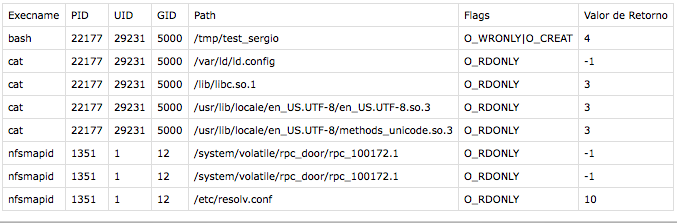
\includegraphics[width=0.5\textwidth]{Tables/cat1.png}
\caption{Resultado Comando \textit{cat /etc/inittab $>$ /tmp/test}}
\label{fig:cat1}
\end{center}
\end{figure}

\item Comando cat /etc/inittab $\gg$ /tmp/test - Ao executarmos este comando estamos a fazer uma leitura do ficheiro \textit{inittab}. Além disso este comando acrescenta o \textit{Output} ao ficheiro \textit{test\_sergio} já existente, como tal é de esperar que na coluna referente às \textit{flags} apareçam as \textit{flags O\_WRONLY, O\_APPEND} e a \textit{flag O\_CREAT}, o que se verifica pela análise da 1ª linha da tabela da figura \ref{fig:cat2}.
\begin{figure}[h!]
\begin{center}
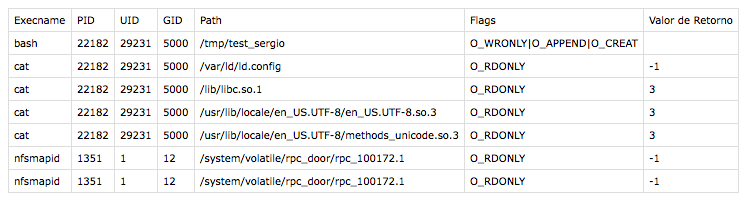
\includegraphics[width=0.5\textwidth]{Tables/cat2.png}
\caption{Resultado Comando cat /etc/inittab $\gg$ /tmp/test}
\label{fig:cat2}
\end{center}
\end{figure}

\item Comando cat /etc/inittab $|$ tee /tmp/test - Ao executarmos este comando a saída do comando \textit{cat /etc/inittab} vai ser gravada no ficheiro \textit{test} ao mesmo tempo em que é exibida no ecrá. O resultado obtido pela execução deste comando pode ser consultado na tabela da figura \ref{fig:cat3}.
\begin{figure}[h!]
\begin{center}
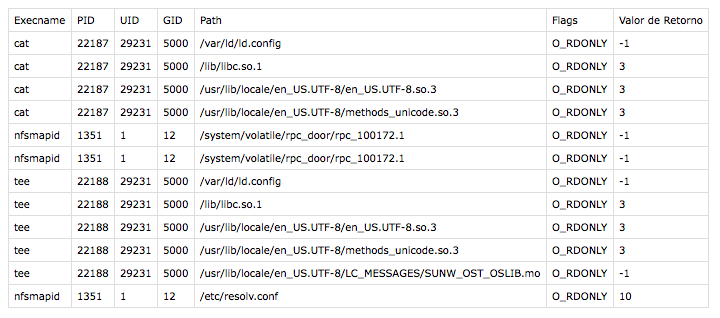
\includegraphics[width=0.5\textwidth]{Tables/cat3.png}
\caption{Resultado Comando cat /etc/inittab $|$ tee /tmp/test}
\label{fig:cat3}
\end{center}
\end{figure}

\item Comando cat /etc/inittab $|$ tee -a /tmp/test - Esfe comando faz exactamente o que faz o comando do tópico anterior, com a diferença que com a \textit{flag -a} este acrescenta a saída do comando \textit{cat /etc/inittab} ao ficheiro \textit{test}. O resultado obtido pela execução deste comando pode ser consultado na tabela da figura \ref{fig:cat4}.
\begin{figure}[h!]
\begin{center}
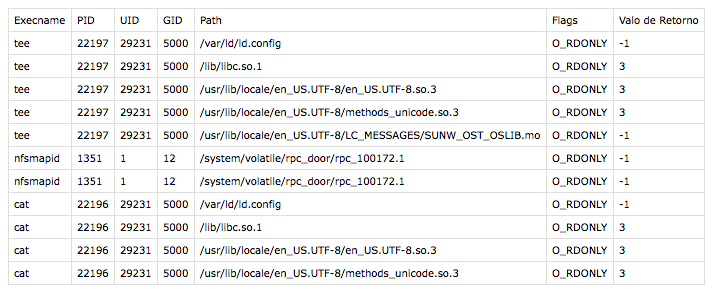
\includegraphics[width=0.5\textwidth]{Tables/cat4.png}
\caption{Resultado Comando cat /etc/inittab $|$ tee -a /tmp/test}
\label{fig:cat4}
\end{center}
\end{figure}

\end{itemize}

\section{Exercicio 2}
Neste exercício, foi-nos proposto criar uma script que para cada processo em execução no sistema mostra-se as seguintes estatísticas:
\begin{itemize}
\item Número de tentativas de abrir ficheiros existentes;
\item Número de tentativas para criar ficheiros;
\item Número de tentativas bem-sucedidas.
\end{itemize}
Estas estatísticas devem ser imprimidas no ecrã, juntamente com a hora e dia, repetidamente, com um período (em segundos) passado como argumento na linha de comandos.

\subsection{Script}

Esta \textit{Script} é constituida por 3 provas,  primeira vai contar o número de tentativas para criar ficheiros, para isso esta prova contém um predicado que testa se a \textit{flag} da chamada ao sistema \textit{openat} é a \textit{flag O\_CREAT}, caso se verifique este predicado é incrementado um contador através de uma agregação com um \textit{array} associativo (\textit{@create[execname,pid]}). As outras duas provas, uma conta o numero de tentativas para abrir um ficheiro e a outra o numero de tentativas bem sucedidas, as ações associadas a estas provas processam-se da mesma forma que foi explicado atrás. No final é imprimido no ecrã o dia e a hora, o nome do executável, o PID, o contador do \textit{array @create}, o contador do \textit{array @open} e o contador do \textit{array @success}, com um período de 2 segundos

\begin{lstlisting}
/* 
inline int O_RDONLY = 0;
inline int O_WRONLY = 1;
inline int O_RDWR = 2;
inline int O_APPEND = 8;
inline int O_CREAT = 256;
*/

syscall::openat:entry
/(arg2 & O_CREAT)==O_CREAT/
{       
        @create[execname,pid] = count();
}

syscall::openat*:entry
/(arg2 & O_CREAT) == 0/ {
         @open[execname, pid] = count();
}
 
syscall::openat*:return
/ arg1 > 0 / {
        @success[execname, pid] = count();
}

tick-$1s
{       
         
         printf ("%Y\n",walltimestamp);
         printf("%12s %6s %6s %6s %s\n","EXECNAME", "PID", "CREATE", "OPEN", "SUCCESS");
         printa ("%12s %6d %@6d %@6d %@d\n", @create, @open, @success);
         trunc(@create);
         trunc(@open); 
         trunc(@success);
}
\end{lstlisting}

\subsection{Resultados Obtidos}

Os resultados obtidos na execução da \textit{script}, referente ao exercício 2, podem ser consultados na figura \ref{fig:ex2}. Estes resultados foram obtidos através da execução do seguinte comando:

\begin{lstlisting}
dtrace -qs exercicio2.d 2
\end{lstlisting}

Sendo que 2, é o período (segundos) pelo qual os resultados são imprimidos no ecrã. De referir que nem sempre as provas detectam alguma coisa, pode haver períodos em que não há nenhuma atividade que satisfaça as provas definidas.

\begin{figure}[H]
\begin{center}
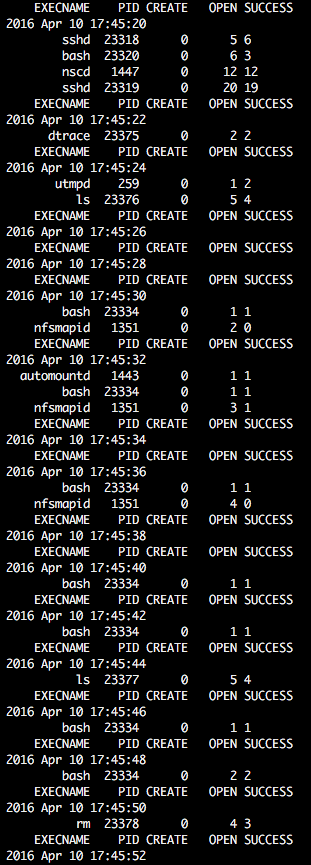
\includegraphics[width=0.5\textwidth]{Tables/ex2.png}
\caption{Resultado da \textit{Script} do Exercicio 2}
\label{fig:ex2}
\end{center}
\end{figure}

\section{Análise de Aplicação Paralela (OpenMP) com Ferramenta Dtrace}

Nesta secção irei analisar, a execução de uma aplicação paralela, fornecida pelo professor, com uma \textit{script} em \textit{Dtrace}. A aplicação em causa é um gerador de números aleatórios, numa gama de um intervalo dado. A aplicação está paralelizada seguindo um paradigma de memória partilhada, mais propriamente com a utilização de pragmas \textit{OpenMP}. O código referente à aplicação fornecida pelo professor pode ser consultado em baixo:

\lstinputlisting[language=C]{ex2_v2.cpp} 

A \textit{script DTrace}, também fornecida pelo professor, permite-nos obter vários tipos de informação relativamente à aplicação em causa. A \textit{script} permite-nos saber quando a \textit{Thread} foi criada e finalizada, em que CPU está a correr (se trocar de CPU também é possível observar essa troca), quando é interrompida e como é interrompida. A \textit{script} em \textit{DTrace} pode ser consultada em baixo:

\lstinputlisting[language=C]{threadshed.d}

O objetivo desta análise passa por analisar o comportamento da aplicação para os diferentes tipos de escalonamento:

\begin{itemize}
	\item \textbf{\textit{static}} - Este tipo de escalonamento divide o ciclo para \textit{chunks} iguais ou o mais igual possível, caso o numero de iterações do ciclo não seja divisível por o número de \textit{Threads} multiplicado pelo tamanho do \textit{chunk}.
	\item \textbf{\textit{dynamic}} - Com este escalonamento é distribuído \textit{chunck's}, com tamanho fixo, pelo numero de \textit{threads} e estes segmentos são organizados numa \textit{queue}. Quando um segmento termina é atribuido outro segmento com o mesmo tamanho. Este tipo de escalonamento tem um \textit{overhead} associado.
	\item \textbf{\textit{guided}} - Este tipo de escalonamento é semelhante ao \textit{dynamic}, contudo o tamanho do \textit{chunk} começa grande e diminuindo de forma a melhorar o balanceamento das cargas entre as iterações. Por defeito o tamanho do \textit{chunk} é aproximadamente $loop\_count/number\_of\_threads$.
\end{itemize}

Para a execução e teste da aplicação criei uma \textit{shell script} em que testei todos os tipos de escalonamento (\textit{static, guided, dynamic}) para um numero variável de \textit{Threads} (1, 2, 4, 8, 16, 32 e 64), recolhendo para cada número de \textit{threads} um total de 10 amostras, das quais escolhi a amostra com melhor tempo.

\subsection{Análise dos Tempos para os Diferentes Tipos de Escalonamento}

No gráfico da figura \ref{fig:sched}, podemos consultar os diferentes tempos para os diferentes tipos de escalonamento para diferentes números de \textit{threads}.

\begin{figure}[H]
\begin{center}
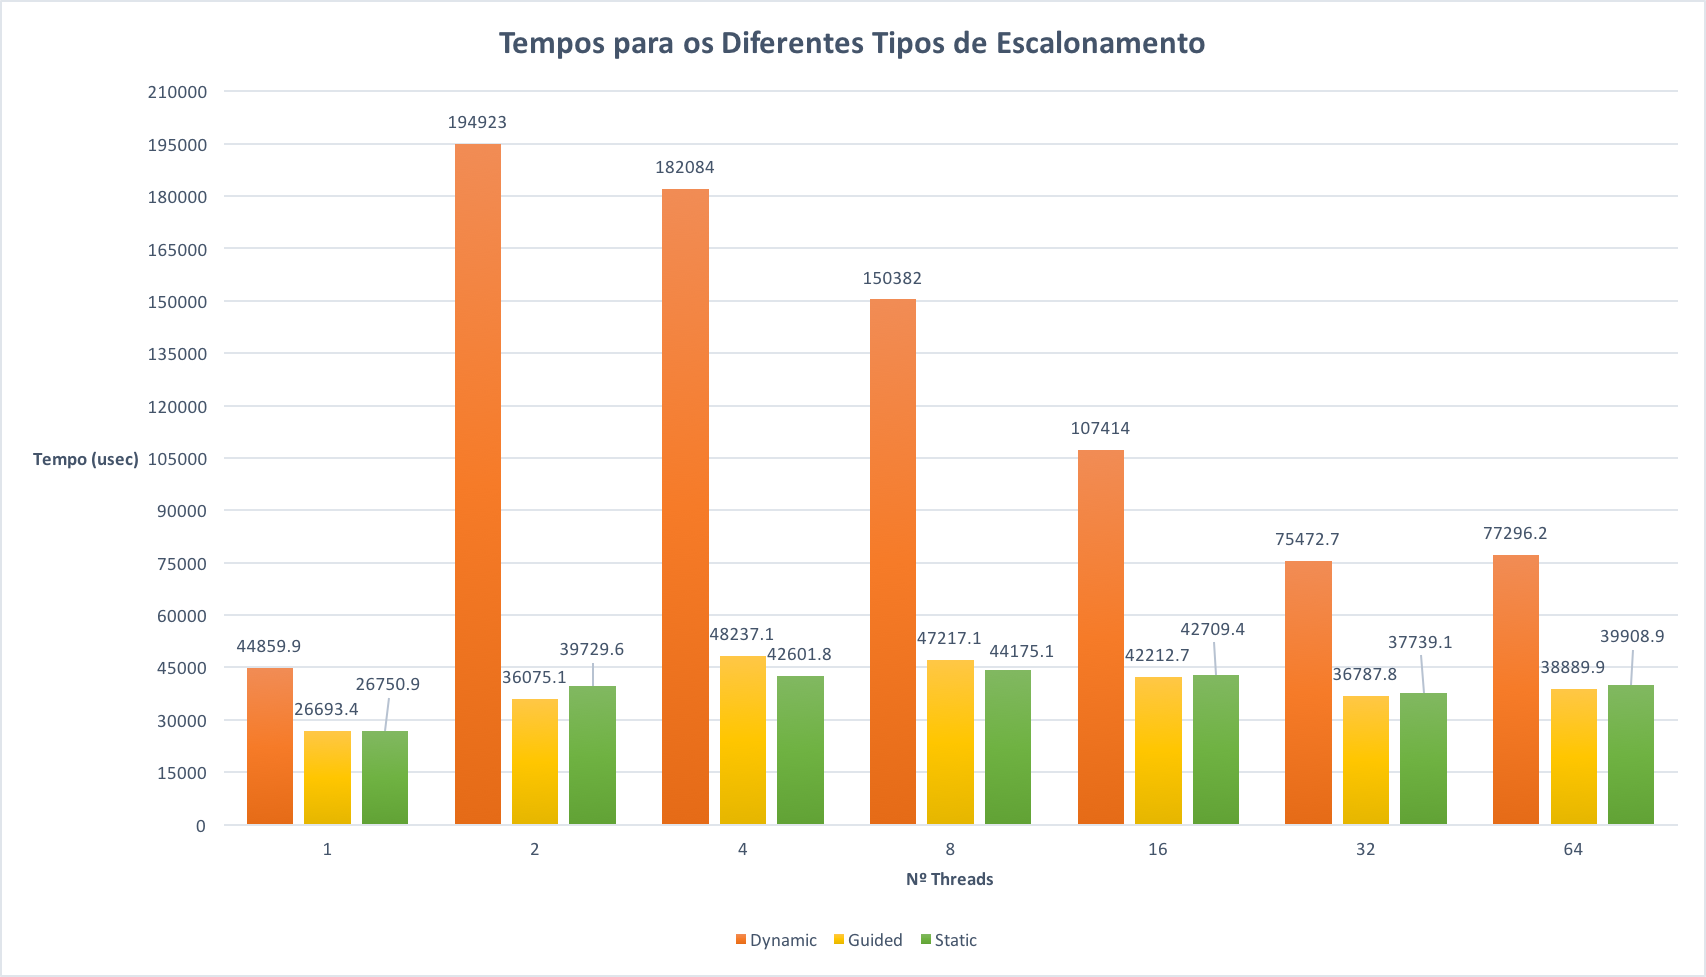
\includegraphics[width=0.5\textwidth]{grafico_tempos.png}
\caption{Tempos para os Diferentes Tipos de Escalonamento para Diferentes Nº de Threads}
\label{fig:sched}
\end{center}
\end{figure}

Ao analisarmos o gráfico, verificamos que o escalonamento \textit{dynamic} é sempre o que apresenta piores tempos, isto pode ser justificado, pelo facto deste escalonamento ter um \textit{overhead} associado. Este \textit{overhead} está associado ao tempo que é necessário para se fazer as divisões das iterações em blocos e posteriormente organiza-las na \textit{queue}.

Quanto aos outros dois tipos de escalonamento (\textit{guided, static}), estes apresentam tempos relativamente iguais à medida que se aumenta o número de \textit{threads}. Como tal não me é possível concluir qual a melhor política de escalonamento em termos de tempo, uma vez que estes tempos são semelhantes para o \textit{static} e para o \textit{guided}.

Relativamente aos resultados obtidos para 64 \textit{threads}, tenho de admitir que os resultados, são surpreendentes, uma vez que quando a aplicação é executada, estamos a usar o dobro das \textit{threads} disponíveis na máquina. Como tal, seria de esperar que os tempos fossem um pouco superiores, uma vez que a máquina está a usar \textit{threads} partilhadas, e como podemos verificar pela a análise do gráfico da figura \ref{fig:sched}, vemos que os tempos continuam mais ao menos semelhantes de quando a aplicação é executada com 32 \textit{threads}.

Fazendo ainda uma análise ao paralelismo da aplicação, podemos verificar que é com a versão sequencial (1 \textit{thread})desta que se obtém o melhor tempo, relativamente ás versões com um maior número de \textit{threads}. O que permite concluir que este código não é o melhor código para ser paralelizado uma vez que o melhor tempo é obtido sequêncialmente. 

\subsection{Análise do Comportamento das Threads para os Diferentes Tipos de Escalonamento}

Para a análise dos resultados, escolhi analisar um excerto do output da \textit{Script Dtrace} da melhor execução, para 32 \textit{threads} para o escalonamento \textit{static} com um intervalo de 100. Escolhi 32 \textit{threads} porque é o número máximo de \textit{threads} suportado pela máquina.

\begin{lstlisting}
	0:0         TID   1 CPU   1(1) created
        0:0         TID   1 CPU   1(1) created
fiosExecucao =32 Intervalo=99
 tempo -> 37739.1 usecs
        9:0         TID   3 CPU   0(1) created
        9:1465575350619 TID   3 CPU   0(1) restarted on the same CPU
        9:1465575350619 TID   3 sleeping on 'cond var'
        9:1465575350619 TID   3 CPU   0(1) preempted
        9:0         TID   7 CPU   0(1) created
        9:1465575350619 TID   7 CPU   0(1) restarted on the same CPU
        9:1465575350619 TID   7 sleeping on 'cond var'
        9:1465575350619 TID   7 CPU   0(1) preempted
        9:0         TID   9 CPU   0(1) created
        9:1465575350619 TID   9 CPU   0(1) restarted on the same CPU
        9:1465575350619 TID   9 sleeping on 'cond var'
        9:1465575350619 TID   9 CPU   0(1) preempted
        9:0         TID  11 CPU   0(1) created
        9:1465575350619 TID  11 CPU   0(1) restarted on the same CPU
        9:1465575350619 TID  11 sleeping on 'cond var'
        9:1465575350619 TID  11 CPU   0(1) preempted
        9:0         TID  13 CPU   0(1) created
        9:1465575350619 TID  13 CPU   0(1) restarted on the same CPU
        9:1465575350619 TID  13 sleeping on 'cond var'
        9:1465575350619 TID  13 CPU   0(1) preempted
        9:0         TID  15 CPU   0(1) created
        9:1465575350619 TID  15 CPU   0(1) restarted on the same CPU
        9:1465575350619 TID  15 sleeping on 'cond var'
        9:1465575350619 TID  15 CPU   0(1) preempted
        9:0         TID  17 CPU   0(1) created
        9:1465575350619 TID  17 CPU   0(1) restarted on the same CPU
        9:1465575350619 TID  17 sleeping on 'cond var'
        9:1465575350619 TID  17 CPU   0(1) preempted
        9:0         TID  19 CPU   0(1) created
        9:1465575350619 TID  19 CPU   0(1) restarted on the same CPU
        9:1465575350619 TID  19 sleeping on 'cond var'
        9:1465575350619 TID  19 CPU   0(1) preempted
        9:0         TID  21 CPU   0(1) created
        9:1465575350619 TID  21 CPU   0(1) restarted on the same CPU
        9:1465575350619 TID  21 sleeping on 'cond var'
        9:1465575350619 TID  21 CPU   0(1) preempted
        9:0         TID  23 CPU   0(1) created
        9:1465575350619 TID  23 CPU   0(1) restarted on the same CPU
        9:1465575350619 TID  23 sleeping on 'cond var'
        9:1465575350619 TID  23 CPU   0(1) preempted
        9:0         TID  25 CPU   0(1) created
        9:1465575350619 TID  25 CPU   0(1) restarted on the same CPU
        9:1465575350619 TID  25 sleeping on 'cond var'
        9:1465575350619 TID  25 CPU   0(1) preempted
        9:0         TID  27 CPU   0(1) created
        9:1465575350619 TID  27 CPU   0(1) restarted on the same CPU
        9:1465575350619 TID  27 sleeping on 'cond var'
        9:1465575350619 TID  27 CPU   0(1) preempted
        9:0         TID  29 CPU   0(1) created
        9:1465575350619 TID  29 CPU   0(1) restarted on the same CPU
        9:1465575350619 TID  29 sleeping on 'cond var'
        9:1465575350619 TID  29 CPU   0(1) preempted
        9:0         TID  31 CPU   0(1) created
        9:1465575350619 TID  31 CPU   0(1) restarted on the same CPU
        9:1465575350619 TID  31 sleeping on 'cond var'
        9:1465575350619 TID  31 CPU   0(1) preempted
        9:1465575350619 TID   7 CPU   0(1) restarted on the same CPU
       39:1465575350649 TID   7 sleeping on 'cond var'
       39:1465575350649 TID   7 CPU   0(1) preempted
       49:1465575350659 TID   7 CPU   0(1) restarted on the same CPU
       49:1465575350659 TID   7 sleeping on 'cond var'
       49:1465575350659 TID   7 CPU   0(1) preempted
       49:1465575350659 TID   7 CPU   0(1) restarted on the same CPU
       49:1465575350659 TID   1  from-CPU 19(1) to-cpu 0(1) CPU migration
       49:1465575350659 TID   1 CPU   0(1) restarted on the same CPU
       49:1465575350659 TID   1 sleeping on 'cond var'
       49:1465575350659 TID   1 CPU   0(1) preempted
       49:1465575350659 TID   1 CPU   0(1) restarted on the same CPU
       49:1465575350659 TID   1 sleeping on 'cond var'
       49:1465575350659 TID   1 CPU   0(1) preempted
       49:1465575350659 TID   1 CPU   0(1) restarted on the same CPU
       49:1465575350659 TID   1 sleeping on 'cond var'
       49:1465575350659 TID   1 CPU   0(1) preempted
\end{lstlisting}

Escolhi apenas este excerto do output para o escalonamento \textit{static} para 32 \textit{threads}, uma vez, que depois da analise dos outros outputs não verifica grandes diferenças.

Como podemos verificar pelo output em cima, as \textit{threads} são criadas, em diferentes CPU's e à medida que o programa é executado, estas por sua vez podem ser interrompidas (\textit{prempted}), ou seja saem do CPU, depois de interrompidas, as \textit{threads} normalmente recomeçam a sua execução no mesmo CPU (\textit{restarted on the same CPU}). 

As \textit{threads} podem ficar adormecidas (\textit{sleeping}), isto acontece porque são forçadas a parar pelas variáveis de condição (\textit{sleeping on 'cond var'} no caso do output apresentado) ficando a espera que haja uma alteração na variável de condição. Estas também podem ser forçadas a parar por \textit{mutex} e a semáforos.

No output apresentado, também podemos verificar que por várias vezes as \textit{threads} podem migrar de um CPU para outro (\textit{from-CPU 19(1) to-cpu 0(1) CPU migration}). 

Como o tipo de escalonamento é \textit{static}, sempre que termina um segmento associado a essa \textit{thread} logo a seguir é atribuído um novo segmento para execução, segmentos esses que têm sempre o mesmo tamanho como já foi referido anteriormente.

Podemos analisar que o aumento do tempo total para a conclusão da aplicação não está directamente associado a tempo "perdido" em \textit{sleep} por, p.e. variáveis de condição ou desafectação forçada. É a própria biblioteca OpenMP que implica uma adição em termos de \textit{overhead} em tempo de computação -- neste traçado incluído nas linhas \textit{restarted on the same CPU}, ou seja, CPU-Time. Não nos é possível distinguir o CPU-TIME despendido em porções de código da aplicação ou na biblioteca OpenMP.

\section{Conclusão}
Como podemos verificar, ao longo deste trabalho, tivemos desenvolver duas scripts que nos permiti-se traçar/detectar o que nos foi pedido no enunciado. Ao longo do desenvolvimento apercebi-me cada vez mais das capacidades da \textit{Framework Dtrace}, sendo que esta ferramenta nos permite, monitorizar ao pormenor tudo o que acontece num sistema. Para além desta grande vantagem, esta ferramenta também apresenta uma linguagem própria, a linguagem \textit{D}, que como já foi referido anteriormente, é uma linguagem muito parecida (estruturalmente) com o \textit{awk}.

Com esta linguagem, a \textit{Framework} torna-se ainda muito mais "poderosa", uma vez que nos permite aproximar até ao máximo detalhe daquilo que pretendemos analisar no sistema.

Em relação ao trabalho extra, sugerido pelo professor no final do semestre, podemos verificar que com uma simples \textit{script Dtrace} podemos fazer um traçado dinâmico do comportamento de todas as \textit{threads} envolvidas na execução da aplicação paralela, para os diferentes tipos de escalonamento. Com esta \textit{script} temos total controlo do percurso de cada \textit{thread} ao longo da toda a execução. Uma vez mais, com este exemplo, podemos apercebermo-nos da potencialidade e utilidade da ferramenta \textit{DTrace}, quer para versões sequências quer para versões paralelas de código.

Como trabalho futuro, pretendo aperfeiçoar os meus conhecimentos em \textit{Dtrace}, porque, como já disse, para além de ser uma ferramenta poderosa, no que toca a administração de sistemas, também é uma ferramenta muito útil e acessível uma vez que a sua sintaxe não é muito difícil nem a sua estrutura, o que se torna difícil no estudo desta ferramenta é a numerosa informação que se dispõem, bem como as numerosas provas que é permitido se criar com o \textit{Dtrace}.
% An example of a floating figure using the graphicx package.
% Note that \label must occur AFTER (or within) \caption.
% For figures, \caption should occur after the \includegraphics.
% Note that IEEEtran v1.7 and later has special internal code that
% is designed to preserve the operation of \label within \caption
% even when the captionsoff option is in effect. However, because
% of issues like this, it may be the safest practice to put all your
% \label just after \caption rather than within \caption{}.
%
% Reminder: the "draftcls" or "draftclsnofoot", not "draft", class
% option should be used if it is desired that the figures are to be
% displayed while in draft mode.
%
%\begin{figure}[!t]
%\centering
%\includegraphics[width=2.5in]{myfigure}
% where an .eps filename suffix will be assumed under latex, 
% and a .pdf suffix will be assumed for pdflatex; or what has been declared
% via \DeclareGraphicsExtensions.
%\caption{Simulation results for the network.}
%\label{fig_sim}
%\end{figure}

% Note that the IEEE typically puts floats only at the top, even when this
% results in a large percentage of a column being occupied by floats.


% An example of a double column floating figure using two subfigures.
% (The subfig.sty package must be loaded for this to work.)
% The subfigure \label commands are set within each subfloat command,
% and the \label for the overall figure must come after \caption.
% \hfil is used as a separator to get equal spacing.
% Watch out that the combined width of all the subfigures on a 
% line do not exceed the text width or a line break will occur.
%
%\begin{figure*}[!t]
%\centering
%\subfloat[Case I]{\includegraphics[width=2.5in]{box}%
%\label{fig_first_case}}
%\hfil
%\subfloat[Case II]{\includegraphics[width=2.5in]{box}%
%\label{fig_second_case}}
%\caption{Simulation results for the network.}
%\label{fig_sim}
%\end{figure*}
%
% Note that often IEEE papers with subfigures do not employ subfigure
% captions (using the optional argument to \subfloat[]), but instead will
% reference/describe all of them (a), (b), etc., within the main caption.
% Be aware that for subfig.sty to generate the (a), (b), etc., subfigure
% labels, the optional argument to \subfloat must be present. If a
% subcaption is not desired, just leave its contents blank,
% e.g., \subfloat[].


% An example of a floating table. Note that, for IEEE style tables, the
% \caption command should come BEFORE the table and, given that table
% captions serve much like titles, are usually capitalized except for words
% such as a, an, and, as, at, but, by, for, in, nor, of, on, or, the, to
% and up, which are usually not capitalized unless they are the first or
% last word of the caption. Table text will default to \footnotesize as
% the IEEE normally uses this smaller font for tables.
% The \label must come after \caption as always.
%
%\begin{table}[!t]
%% increase table row spacing, adjust to taste
%\renewcommand{\arraystretch}{1.3}
% if using array.sty, it might be a good idea to tweak the value of
% \extrarowheight as needed to properly center the text within the cells
%\caption{An Example of a Table}
%\label{table_example}
%\centering
%% Some packages, such as MDW tools, offer better commands for making tables
%% than the plain LaTeX2e tabular which is used here.
%\begin{tabular}{|c||c|}
%\hline
%One & Two\\
%\hline
%Three & Four\\
%\hline
%\end{tabular}
%\end{table}


% Note that the IEEE does not put floats in the very first column
% - or typically anywhere on the first page for that matter. Also,
% in-text middle ("here") positioning is typically not used, but it
% is allowed and encouraged for Computer Society conferences (but
% not Computer Society journals). Most IEEE journals/conferences use
% top floats exclusively. 
% Note that, LaTeX2e, unlike IEEE journals/conferences, places
% footnotes above bottom floats. This can be corrected via the
% \fnbelowfloat command of the stfloats package.




% trigger a \newpage just before the given reference
% number - used to balance the columns on the last page
% adjust value as needed - may need to be readjusted if
% the document is modified later
%\IEEEtriggeratref{8}
% The "triggered" command can be changed if desired:
%\IEEEtriggercmd{\enlargethispage{-5in}}

% references section

% can use a bibliography generated by BibTeX as a .bbl file
% BibTeX documentation can be easily obtained at:
% http://mirror.ctan.org/biblio/bibtex/contrib/doc/
% The IEEEtran BibTeX style support page is at:
% http://www.michaelshell.org/tex/ieeetran/bibtex/
%\bibliographystyle{IEEEtran}
% argument is your BibTeX string definitions and bibliography database(s)
%\bibliography{IEEEabrv,../bib/paper}
%
% <OR> manually copy in the resultant .bbl file
% set second argument of \begin to the number of references
% (used to reserve space for the reference number labels box)

\bibliographystyle{abbrv}
\bibliography{ref.bib}


% that's all folks
\end{document}


